\setmonofont[Path=fonts/,Scale=0.90,BoldFont={SourceCodePro-Bold}]{SourceCodePro-Regular}
%% Fontfeatures after setting the mono font to keep
%% lstlisting fonts happy
%%\defaultfontfeatures{Scale=MatchLowercase,Mapping=tex-text}
\defaultfontfeatures{Mapping=tex-text}
\setmainfont[Path=fonts/,ItalicFont={PTS56F},BoldFont={PTS75F}]{PTS55F}
\def\inputGnumericTable{}

\setulmarginsandblock{2.5cm}{2.5cm}{*}
\checkandfixthelayout
\setlength{\textwidth}{1.1\textwidth}
\setlength{\parindent}{0pt}
\setlength{\parskip}{0.7ex plus 0.5ex minus 0.2ex}

%% list of answers
\newlistof{listofex}{ex}{List of Exercises}
\newlistentry{exercise}{ex}{0}

\renewcommand{\tocheadstart}{}
\renewcommand{\aftertoctitle}{\pagestyle{blocks}}
\renewcommand{\aftertoctitle}{\thispagestyle{empty}\afterchaptertitle\pagestyle{blocks}}

%%\renewcommand{\printtoctitle}[1]{}
\renewcommand{\contentsname}{Contents}
\renewcommand{\tocmark}{\markboth{\myfamily \typename: \contentsname}{\myfamily \contentsname}}
%% new print the titles as section not as chapter, that explains
%% why the page is headerless. the page style is empty
%% lof
\renewcommand{\lofheadstart}{}
\renewcommand{\afterloftitle}{\thispagestyle{blocks}}
\renewcommand{\printloftitle}[1]{\section*{#1}}
\renewcommand{\lotmark}{\markboth{\myfamily \typename:
\contentsname}{\myfamily \listfigurename}}
%% lot
\renewcommand{\lotheadstart}{}
\renewcommand{\afterlottitle}{\thispagestyle{blocks}}
\renewcommand{\printlottitle}[1]{\section*{#1}}
\renewcommand{\lofmark}{\markboth{\myfamily \typename:
\contentsname}{\myfamily \listtablename}}
%% ex
\renewcommand{\exheadstart}{}
\renewcommand{\afterextitle}{\thispagestyle{blocks}}
\renewcommand{\printextitle}[1]{\section*{#1}}
\renewcommand{\exmark}{\markboth{\myfamily \typename: \contentsname}{\myfamily List of Exercises}}

\nobibintoc
\renewcommand*{\indexmark}{%
\markboth{\myfamily \typename{} \thechapter: \indexname}{\myfamily\indexname}%
}

\onecolindexfalse  %% doesn't do its things as advertised
\noindexintoc
\makeindex

%% make quote print italics
\newcommand{\qquote}{{\scalefont{4.00}{``}}}
\expandafter\def\expandafter\quote\expandafter{\quote\em}

%% Listings
\newfontfamily\listingsfont[Path=fonts/,Scale=0.90,BoldFont={SourceCodePro-Bold}]{SourceCodePro-Regular}

\lstdefinelanguage{Go}
  {morekeywords={append,break,cap,case,chan,const,continue,copy,default,defer,else,fallthrough,%
  for,func,go,goto,if,import,interface,len,make,map,new,package,range,return,select,%
  struct,switch,type,var,%  % types
  uint8,uint16,uint32,uint64,int8,int16,int32,int64,float32,float64,byte,%
  complex,complex128,complex64,%
  int,rune,uint,bool,uintptr,string,%
  error,iota,%
  },%
  otherkeywords={<-,!,;,\{,\}},%  %% nog beter maken
    sensitive=true,%
    morecomment=[l]{//},%
    morecomment=[s]{/*}{*/},%
    morecomment=[n]{(*}{*)},%
    morestring=[b]",%
    morestring=[b]',%
    morestring=[b]`,%
  }[]%
\lstset{language=Go,inputencoding=utf8,extendedchars=false,texcl,escapechar=\|,basicstyle=\ttfamily,keywordstyle=\normalfont,numbers=none,numberblanklines=false,showstringspaces=false,breaklines=true,numberstyle=\small\ttfamily,xleftmargin=\parindent,xrightmargin=1em,linewidth=0.98\linewidth}
%,literate={"}{\textasciiquote}{1}}

\newcommand{\coderemark}[1]{\sffamily\qquad$\leftarrow \textit{\footnotesize #1}$}

%% Cite style
%%\bibpunct{[}{]}{;}{s}{,}{,}

%% Exercises
\renewcommand{\ExerciseHeaderTitle}{\ExerciseTitle}
\renewcommand{\ExerciseHeaderLabel}{}
\renewcommand{\ExerciseName}{}	%% was 'Exercise'
\renewcommand{\ExerciseHeaderNB}{\theExercise}
%% This one is actually used
\renewcommand{\ExerciseHeader}{\vspace{.7ex}\noindent\textbf{Q\theExercise}. (\number\ExerciseDifficulty) \ExerciseTitle\quad%
\addcontentsline{ex}{exercise}{\numberline{\theExercise}(\number\ExerciseDifficulty) \ExerciseTitle}}
\renewcommand{\AnswerHeader}{\vspace{.7ex}\noindent\textbf{A\theExercise}.  (\number\ExerciseDifficulty) \ExerciseTitle\quad}

%% Style commands
\newcommand{\func}[1]{\texttt{#1}}
\newcommand{\key}[1]{\texttt{#1}}
\newcommand{\type}[1]{\texttt{#1}}
\newcommand{\prog}[1]{\texttt{#1}}
\newcommand{\flag}[1]{\textit{#1}}
\newcommand{\dir}[1]{\texttt{#1}}
\newcommand{\file}[1]{\texttt{#1}}
\newcommand{\var}[1]{\texttt{#1}}
\newcommand{\rem}[1]{\texttt{\textit{#1}}}
\newcommand{\package}[1]{{\textit{#1}}}
\newcommand{\first}[2]{#1\index{#2}}
\newcommand{\error}[1]{\texttt{#1}}
\newcommand{\pr}{\%}           %% a prompt (also bold)
\newcommand{\user}[1]{\textbf{#1}}      %% text a user should type
\newcommand{\userinput}[1]{\textit{#1}} %% text a user should choose
\newcommand{\gorelease}[1]{\texttt{#1}}

%% Footnotes
\renewcommand*{\thefootnote}{\textbf{\emph\alph{footnote}}}

%% Epigraph
\newcommand{\epi}[2]{\epigraph{#1}{#2}}
\setlength{\epigraphwidth}{1.2\epigraphwidth}

%% Margin notes
\setmarginnotes{0.04\stockwidth}{0.12\stockwidth}{\onelineskip}
\newcommand{\gomarginpar}[1]{%
\marginpar{\itshape\small#1}}
%% typeset text in margin and index arg 2
\newcommand{\gomarginindex}[2]{\gomarginpar{#1}\index{#2}}
\newcommand{\gopher}{%
\begin{figure}[H]%
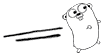
\includegraphics[scale=0.20, width=.70\marginparwidth]{fig/gopher.png}%
\end{figure}%
}

\setCJKmainfont{AR PL UKai CN}

\newcommand{\ubrace}[3]{%
\draw [thick,decorate,decoration={brace,amplitude=4pt},xshift=0pt,yshift=0pt] %
(#1) -- (#2) node [black,midway,below=4pt,xshift=0pt] %
{\longremark{#3}}; %
}

%% fixes
\newcommand{\exdisfix}{\vspace{1ex}}
